% ------------------------------------------------------------
% LaTeX Template für die DHBW zum Schnellstart!
% Original: https://github.wdf.sap.corp/vtgermany/LaTeX-Template-DHBW
% ------------------------------------------------------------
% ---- Präambel mit Angaben zum Dokument
\documentclass[
	fontsize=12pt,           % Leitlinien sprechen von Schriftgröße 12.
	paper=A4,
	twoside=false,
	listof=totoc,            % Tabellen- und Abbildungsverzeichnis ins Inhaltsverzeichnis
	bibliography=totoc,      % Literaturverzeichnis ins Inhaltsverzeichnis aufnehmen
	titlepage,               % Titlepage-Umgebung anstatt \maketitle
	headsepline,             % horizontale Linie unter Kolumnentitel
	abstract,              % Überschrift einschalten, Abstract muss in {abstract}-Umgebung stehen
]{scrreprt}                  % Verwendung von KOMA-Report
\usepackage[utf8]{inputenc}  % UTF8 Encoding einschalten
\usepackage[ngerman]{babel}  % Neue deutsche Rechtschreibung
\usepackage[T1]{fontenc}     % Ausgabe von westeuropäischen Zeichen (auch Umlaute)
\usepackage{microtype}       % Trennung von Wörtern wird besser umgesetzt
\usepackage{lmodern}         % Nicht-gerasterte Schriftarten (bei MikTeX erforderlich)
\usepackage{graphicx}        % Einbinden von Grafiken erlauben
\usepackage{wrapfig}         % Grafiken fließend im Text
\usepackage{setspace}        % Zeilenabstand \singlespacing, \onehalfspaceing, \doublespacing
\usepackage[
	%showframe,                % Ränder anzeigen lassen
	left=2.7cm, right=2.5cm,
	top=2.5cm,  bottom=2.5cm,
	includeheadfoot
]{geometry}                      % Seitenlayout einstellen
\usepackage{scrlayer-scrpage}    % Gestaltung von Fuß- und Kopfzeilen
\usepackage{acronym}             % Abkürzungen, Abkürzungsverzeichnis
\usepackage{titletoc}            % Anpassungen am Inhaltsverzeichnis
\contentsmargin{0.75cm}          % Abstand im Inhaltsverzeichnis zw. Punkt und Seitenzahl
\usepackage[                     % Klickbare Links (enth. auch "nameref", "url" Package)
  hidelinks,                     % Blende die "URL Boxen" aus.
  breaklinks=true                % Breche zu lange URLs am Zeilenende um
]{hyperref}
\usepackage[hypcap=true]{caption}% Anker Anpassung für Referenzen
\urlstyle{same}                  % Aktuelle Schrift auch für URLs
% Anpassung von autoref für Gleichungen (ergänzt runde Klammern) und Algorithm.
% Anstatt "Listing" kann auch z.B. "Code-Ausschnitt" verwendet werden. Dies sollte
% jedoch synchron gehalten werden mit \lstlistingname (siehe weiter unten).
\addto\extrasngerman{%
	\def\equationautorefname~#1\null{Gleichung~(#1)\null}
	\def\lstnumberautorefname{Zeile}
	\def\lstlistingautorefname{Listing}
	\def\algorithmautorefname{Algorithmus}
	% Damit einheitlich "Abschnitt 1.2[.3]" verwendet wird und nicht "Unterabschnitt 1.2.3"
	% \def\subsectionautorefname{Abschnitt}
}

% ---- Abstand verkleinern von der Überschrift 
\renewcommand*{\chapterheadstartvskip}{\vspace*{.5\baselineskip}}

% Hierdurch werden Schusterjungen und Hurenkinder vermieden, d.h. einzelne Wörter
% auf der nächsten Seite oder in einer einzigen Zeile.
% LaTeX kann diese dennoch erzeugen, falls das Layout ansonsten nicht umsetzbar ist.
% Diese Werte sind aber gute Startwerte.
\widowpenalty10000
\clubpenalty10000

% ---- Für das Quellenverzeichnis
\usepackage[
	backend = biber,                % Verweis auf biber
	language = auto,
	style = numeric,                % Nummerierung der Quellen mit Zahlen
	sorting = none,                 % none = Sortierung nach der Erscheinung im Dokument
	sortcites = true,               % Sortiert die Quellen innerhalb eines cite-Befehls
	block = space,                  % Extra Leerzeichen zwischen Blocks
	hyperref = true,                % Links sind klickbar auch in der Quelle
	%backref = true,                % Referenz, auf den Text an die zitierte Stelle
	bibencoding = auto,
	giveninits = true,              % Vornamen werden abgekürzt
	doi=false,                      % DOI nicht anzeigen
	isbn=false,                     % ISBN nicht anzeigen
    alldates=short                  % Datum immer als DD.MM.YYYY anzeigen
]{biblatex}
\addbibresource{Inhalt/literatur.bib}
\setcounter{biburlnumpenalty}{3000}     % Umbruchgrenze für Zahlen
\setcounter{biburlucpenalty}{6000}      % Umbruchgrenze für Großbuchstaben
\setcounter{biburllcpenalty}{9000}      % Umbruchgrenze für Kleinbuchstaben
\DeclareNameAlias{default}{family-given}  % Nachname vor dem Vornamen
\AtBeginBibliography{\renewcommand{\multinamedelim}{\addslash\space
}\renewcommand{\finalnamedelim}{\multinamedelim}}  % Schrägstrich zwischen den Autorennamen
\DefineBibliographyStrings{german}{
  urlseen = {Einsichtnahme:},                      % Ändern des Titels von "besucht am"
}
\usepackage[babel,german=quotes]{csquotes}         % Deutsche Anführungszeichen + Zitate


% ---- Für Mathevorlage
\usepackage{amsmath}    % Erweiterung vom Mathe-Satz
\usepackage{amssymb}    % Lädt amsfonts und weitere Symbole
\usepackage{MnSymbol}   % Für Symbole, die in amssymb nicht enthalten sind.


% ---- Für Quellcodevorlage
\usepackage{scrhack}                    % Hack zur Verw. von listings in KOMA-Script
\usepackage{listings}                   % Darstellung von Quellcode
\usepackage{xcolor}                     % Einfache Verwendung von Farben
% -- Eigene Farben für den Quellcode
\definecolor{JavaLila}{rgb}{0.4,0.1,0.4}
\definecolor{JavaGruen}{rgb}{0.3,0.5,0.4}
\definecolor{JavaBlau}{rgb}{0.0,0.0,1.0}
\definecolor{ABAPKeywordsBlue}{HTML}{6000ff}
\definecolor{ABAPCommentGrey}{HTML}{808080}
\definecolor{ABAPStringGreen}{HTML}{4da619}
\definecolor{PyKeywordsBlue}{HTML}{0000AC}
\definecolor{PyCommentGrey}{HTML}{808080}
\definecolor{PyStringGreen}{HTML}{008080}
% -- Farben für ABAP CDS
\definecolor{CDSString}{HTML}{FF8C00}
\definecolor{CDSKeywords}{HTML}{6000ff}
\definecolor{CDSAnnotation}{HTML}{00BFFF}
\definecolor{CDSComment}{HTML}{808080}
\definecolor{CDSFunc}{HTML}{FF0000}

% -- Default Listing-Styles

\lstset{
	% Das Paket "listings" kann kein UTF-8. Deswegen werden hier 
	% die häufigsten Zeichen definiert (ä,ö,ü,...)
	literate=%
		{á}{{\'a}}1 {é}{{\'e}}1 {í}{{\'i}}1 {ó}{{\'o}}1 {ú}{{\'u}}1
		{Á}{{\'A}}1 {É}{{\'E}}1 {Í}{{\'I}}1 {Ó}{{\'O}}1 {Ú}{{\'U}}1
		{à}{{\`a}}1 {è}{{\`e}}1 {ì}{{\`i}}1 {ò}{{\`o}}1 {ù}{{\`u}}1
		{À}{{\`A}}1 {È}{{\'E}}1 {Ì}{{\`I}}1 {Ò}{{\`O}}1 {Ù}{{\`U}}1
		{ä}{{\"a}}1 {ë}{{\"e}}1 {ï}{{\"i}}1 {ö}{{\"o}}1 {ü}{{\"u}}1
		{Ä}{{\"A}}1 {Ë}{{\"E}}1 {Ï}{{\"I}}1 {Ö}{{\"O}}1 {Ü}{{\"U}}1
		{â}{{\^a}}1 {ê}{{\^e}}1 {î}{{\^i}}1 {ô}{{\^o}}1 {û}{{\^u}}1
		{Â}{{\^A}}1 {Ê}{{\^E}}1 {Î}{{\^I}}1 {Ô}{{\^O}}1 {Û}{{\^U}}1
		{œ}{{\oe}}1 {Œ}{{\OE}}1 {æ}{{\ae}}1 {Æ}{{\AE}}1 {ß}{{\ss}}1
		{ű}{{\H{u}}}1 {Ű}{{\H{U}}}1 {ő}{{\H{o}}}1 {Ő}{{\H{O}}}1
		{ç}{{\c c}}1 {Ç}{{\c C}}1 {ø}{{\o}}1 {å}{{\r a}}1 {Å}{{\r A}}1
		{€}{{\euro}}1 {£}{{\pounds}}1 {«}{{\guillemotleft}}1
		{»}{{\guillemotright}}1 {ñ}{{\~n}}1 {Ñ}{{\~N}}1 {¿}{{?`}}1,
	breaklines=true,        % Breche lange Zeilen um 
	breakatwhitespace=true, % Wenn möglich, bei Leerzeichen umbrechen
	% Symbol für Zeilenumbruch einfügen
	prebreak=\raisebox{0ex}[0ex][0ex]{\ensuremath{\rhookswarrow}},
	postbreak=\raisebox{0ex}[0ex][0ex]{\ensuremath{\rcurvearrowse\space}},
	tabsize=4,                                 % Setze die Breite eines Tabs
	basicstyle=\ttfamily\small,                % Grundsätzlicher Schriftstyle
	columns=fixed,                             % Besseres Schriftbild
	numbers=left,                              % Nummerierung der Zeilen
	%frame=single,                             % Umrandung des Codes
	showstringspaces=false,                    % Keine Leerzeichen hervorheben
	keywordstyle=\color{blue},
	ndkeywordstyle=\bfseries\color{darkgray},
	identifierstyle=\color{black},
	commentstyle=\itshape\color{JavaGruen},   % Kommentare in eigener Farbe
	stringstyle=\color{JavaBlau},             % Strings in eigener Farbe,
	captionpos=b,                             % Bild*unter*schrift
	xleftmargin=5.0ex
}

% ---- Eigener JAVA-Style für den Quellcode
\renewcommand{\ttdefault}{pcr}               % Schriftart, welche auch fett beinhaltet
\lstdefinestyle{EigenerJavaStyle}{
	language=Java,                             % Syntax Highlighting für Java
	%frame=single,                             % Umrandung des Codes
	keywordstyle=\bfseries\color{JavaLila},    % Keywords in eigener Farbe und fett
	commentstyle=\itshape\color{JavaGruen},    % Kommentare in eigener Farbe und italic
	stringstyle=\color{JavaBlau}               % Strings in eigener Farbe
}

% ---- Eigener ABAP-Style für den Quellcode
\renewcommand{\ttdefault}{pcr}
\lstdefinestyle{EigenerABAPStyle}{
	language=[R/3 6.10]ABAP,
	morestring=[b]\|,                          % Für Pipe-Strings
	morestring=[b]\`,                          % für Backtick-Strings
	keywordstyle=\bfseries\color{ABAPKeywordsBlue},
	commentstyle=\itshape\color{ABAPCommentGrey},
	stringstyle=\color{ABAPStringGreen},
	tabsize=2,
	morekeywords={
		types,
		@data,
		as,
		lower,
		start,
		selection,
		order,
		by,
		inner,
		join,
		key,
		end,
		cast
	}
}

% ---- Eigener Python-Style für den Quellcode
\renewcommand{\ttdefault}{pcr}
\lstdefinestyle{EigenerPythonStyle}{
	language=Python,
	columns=flexible,
	keywordstyle=\bfseries\color{PyKeywordsBlue},
	commentstyle=\itshape\color{PyCommentGrey},
	stringstyle=\color{PyStringGreen}
}

%----- ABAP-CDS-View language
\lstdefinelanguage{ABAPCDS}{
	sensitive=false,
	%Keywords
	morekeywords={define,
		view,
		as,
		select,
		from,
		inner,
		join,
		on,
		key,
		case,
		when,
		then,
		else,
		end,
		true,
		false,
		cast,
		where,
		and,
		distinct,
		group,
		by,
		having,
		min,
		sum,
		max,
		count,
		avg
	},
	%Methoden
	morekeywords=[2]{
		div,
		currency\_conversion,
		dats\_days\_between,
		concat\_with\_space,
		dats\_add_days,
		dats\_is\_valid,
		dats\_add\_months,
		unit\_conversion,
		division,
		mod,
		abs,
		floor,
		ceil,
		round,
		concat,
		replace,
		substring,
		left,
		right,
		length
	},
	morecomment=[s][\color{CDSAnnotation}]{@}{:},
	morecomment=[l][\itshape\color{CDSComment}]{//},
	morecomment=[s][\itshape\color{CDSComment}]{/*}{*/},
	morestring=[b][\color{CDSString}]',
	keywordstyle=\bfseries\color{CDSKeywords},
	keywordstyle=[2]\color{CDSFunc}
}

  % Weitere Details sind ausgelagert

\usepackage{algorithm}                  % Für Algorithmen-Umgebung (ähnlich wie lstlistings Umgebung)
\usepackage{algpseudocode}              % Für Pseudocode. Füge "[noend]" hinzu, wenn du kein "endif",
                                        % etc. haben willst.

\makeatletter                           % Sorgt dafür, dass man @ in Namen verwenden kann.
                                        % Ansonsten gibt es in der nächsten Zeile einen Compilefehler.
\renewcommand{\ALG@name}{Algorithmus}   % Umbenennen von "Algorithm" im Header der Listings.
\makeatother                            % Zeichen wieder zurücksetzen
\renewcommand{\lstlistingname}{Listing} % Erlaubt das Umbenennen von "Listing" in anderen Titel.

% ---- Tabellen
\usepackage{booktabs}  % Für schönere Tabellen. Enthält neue Befehle wie \midrule
\usepackage{multirow}  % Mehrzeilige Tabellen
\usepackage{siunitx}   % Für SI Einheiten und das Ausrichten Nachkommastellen
\sisetup{locale=DE, range-phrase={~bis~}, output-decimal-marker={,}} % Damit ein Komma und kein Punkt verwendet wird.
\usepackage{xfrac} % Für siunitx Option "fraction-function=\sfrac"

% ---- Für Definitionsboxen in der Einleitung
\usepackage{amsthm}                     % Liefert die Grundlagen für Theoreme
\usepackage[framemethod=tikz]{mdframed} % Boxen für die Umrandung
% ---- Definition für Highlight Boxen

% ---- Grundsätzliche Definition zum Style
\newtheoremstyle{defi}
  {\topsep}         % Abstand oben
  {\topsep}         % Abstand unten
  {\normalfont}     % Schrift des Bodys
  {0pt}             % Einschub der ersten Zeile
  {\bfseries}       % Darstellung von der Schrift in der Überschrift
  {:}               % Trennzeichen zwischen Überschrift und Body
  {.5em}            % Abstand nach dem Trennzeichen zum Body Text
  {\thmname{#3}}    % Name in eckigen Klammern
\theoremstyle{defi}

% ------ Definition zum Strich vor eines Texts
\newmdtheoremenv[
  hidealllines = true,       % Rahmen komplett ausblenden
  leftline = true,           % Linie links einschalten
  innertopmargin = 0pt,      % Abstand oben
  innerbottommargin = 4pt,   % Abstand unten
  innerrightmargin = 0pt,    % Abstand rechts
  linewidth = 3pt,           % Linienbreite
  linecolor = gray!40,       % Linienfarbe
]{defStrich}{Definition}     % Name der des formats "defStrich"

% ------ Definition zum Eck-Kasten um einen Text
\newmdtheoremenv[
  hidealllines = true,
  innertopmargin = 6pt,
  linecolor = gray!40,
  singleextra={              % Eck-Markierungen für die Definition
    \draw[line width=3pt,gray!50,line cap=rect] (O|-P) -- +(1cm,0pt);
    \draw[line width=3pt,gray!50,line cap=rect] (O|-P) -- +(0pt,-1cm);
    \draw[line width=3pt,gray!50,line cap=rect] (O-|P) -- +(-1cm,0pt);
    \draw[line width=3pt,gray!50,line cap=rect] (O-|P) -- +(0pt,1cm);
  }
]{defEckKasten}{Definition}  % Name der des formats "defEckKasten"  % Weitere Details sind ausgelagert

% ---- Für Todo Notes
\usepackage{todonotes}
\setlength {\marginparwidth }{2cm}      % Abstand für Todo Notizen

\usepackage[htt]{hyphenat}
\usepackage{dirtree,array}
\renewcommand\DTstyle{\fontsize{9}{11}\rmfamily}


% ---- Elektronische Version oder Gedruckte Version?
% ---- Unterschied: Die elektronische Version enthält keinen Platzhalter für die Unterschrift
\usepackage{ifthen}
\newboolean{e-Abgabe}
\setboolean{e-Abgabe}{false}    % false=gedruckte Fassung

% ---- Persönlichen Daten:
\newcommand{\titelheader}{Programmentwurf}
\newcommand{\bearbeitende}{Andr\'{e} Trump und Erik Imgrund}

% ---- Metainformation für das PDF Dokument
\hypersetup{
	pdftitle    = {Software Engineering II (TINF19B1)},
	pdfsubject  = {Programmentwurf},
	pdfauthor   = {\bearbeitende},
	%pdfkeywords = {Keywords angeben},
	pdfcreator  = {LaTeX},
	%pdfproducer = {in der Regel pdfTeX}
}

% ---- Definition der Kopf- und Fußzeilen
\clearpairofpagestyles                          % Löschen von LaTeX Standard
\automark[section]{chapter}                     % Füllen von section und chapter
\renewcommand*{\chaptermarkformat}{}            % Entfernt die Kapitelnummer
\renewcommand*{\sectionmarkformat}{}            % Entfernt die Sectionnummer
% Angaben [für "plain"]{für "scrheadings"}
\ihead[]{\titelheader}                          % Kopfzeile links
\chead[]{}                                      % Kopfzeile mitte
\ohead[]{\rightmark}                            % Kopfzeile rechts
\ifoot[]{}                                      % Fußzeile links
\cfoot*{\sffamily\pagemark}                     % Fußzeile mitte
\ofoot[]{}                                      % Fußzeile rechts
\KOMAoptions{
   headsepline = 0.2pt,                         % Liniendicke Kopfzeile
   footsepline = false                          % Liniendicke Fußzeile
}


% ---- Hilfreiches
\newcommand{\zB}{z.\,B. }   % "z.B." mit kleinem Leeraum dazwischen (ohne wäre nicht korrekt)
\newcommand{\dash}{d.\,h. }

\newcommand{\code}[1]{\texttt{#1}} % Ist einfacher zu schreiben als ständig \texttt und erlaubt
                                   % Änderungen im Nachhinein, wenn man z.B. Inline-Code anders stylen möchte.

% ---- Silbentrennung (falls LaTeX defaults falsch / nicht gewünscht sind)
\hyphenation{HANA}         % anstatt HA-NA
\hyphenation{Graph-Script} % anstatt GraphS-cript

% ---- Beginn des Dokuments
\begin{document}
\setlength{\parindent}{0pt}              % Keine Paragraphen Einrückung.
                                         % Dafür haben wir den Abstand zwischen den Paragraphen.
\setcounter{secnumdepth}{2}              % Nummerierungstiefe fürs Inhaltsverzeichnis
\setcounter{tocdepth}{1}                 % Tiefe des Inhaltsverzeichnisses. Ggf. so anpassen,
                                         % dass das Verzeichnis auf eine Seite passt.
\sffamily                                % Serifenlose Schrift verwenden.

% ---- Vorspann
% ------ Titelseite
\singlespacing
\thispagestyle{empty}
\begin{titlepage}
\enlargethispage{4cm}

\begin{figure}           % Logo vom Ausbildungsbetrieb und der DHBW
	% \vspace*{-5mm} % Sollte dein Titel zu lang werden, kannst du mit diesem "Hack" 
	%                  den Inhalt der Seite nach oben schieben.
	\begin{minipage}{0.49\textwidth}
		\flushleft
		%\includegraphics[width=0.9\textwidth]{Bilder/Logos/Logo.pdf} 
	\end{minipage}
	\hfill
	\begin{minipage}{0.49\textwidth}
		\flushright
		
\includegraphics[height=2.5cm]{Bilder/Logos/Logo_DHBW.pdf} 
	\end{minipage}
\end{figure} 
\vspace*{0.1cm}

\begin{center}
	\huge{\textbf{Software-Engineering II}}\\[1.5cm]
	\Large{\textbf{Programmentwurf}}\\
	\Large{\textbf{TINF19B1}}\\
	\Large{\textbf{5.$+$6. Semester (2021/2022)}}\\[1cm]
	\Large{\textbf{Thema:}}\\
	\Large{\textbf{Matching von Kochrezepten}}\\[2cm]
\end{center}

\begin{center}
	\normalsize{Dozent:}\\
	\large{Daniel Lindner}
\end{center}

\begin{center}
	\normalsize{Bearbeitende:}\\
	\Large{\bearbeitende}
\end{center}
\end{titlepage}
  % Titelseite
\newcounter{savepage}
\pagenumbering{Roman}                    % Römische Seitenzahlen
\onehalfspacing

% ------ Inhaltsverzeichnis
\singlespacing
\tableofcontents

% ------ Verzeichnisse
\renewcommand*{\chapterpagestyle}{plain}
\pagestyle{plain}
\chapter*{Abkürzungsverzeichnis}
\addcontentsline{toc}{chapter}{Abkürzungsverzeichnis} % Hinzufügen zum Inhaltsverzeichnis 

\begin{acronym}[WYSISWG] % längstes Kürzel wird verw. für den Abstand zw. Kürzel u. Text

	% Alphabetisch selbst sortieren - nicht verwendete Kürzel rausnehmen!
	\acro{CLI}{Command Line Interface}
    \acro{JPA}{Java Persistence API}

\end{acronym}

\listoffigures                          % Erzeugen des Abbildungsverzeichnisses 
\renewcommand{\lstlistlistingname}{Quellcodeverzeichnis}
\lstlistoflistings                      % Erzeugen des Listenverzeichnisses
\setcounter{savepage}{\value{page}}


% ---- Inhalt der Arbeit
\cleardoublepage
\pagenumbering{arabic}                  % Arabische Seitenzahlen für den Hauptteil
\setlength{\parskip}{0.5\baselineskip}  % Abstand zwischen Absätzen
\rmfamily
\renewcommand*{\chapterpagestyle}{scrheadings}
\pagestyle{scrheadings}
\onehalfspacing
\chapter{Beschreibung des Programms}
Im Internet ist eine Vielzahl an Rezepten zu finden, welche eine große Unterstützung beim Kochen und eine Erweiterung des eigenen kulinarischen Horizonts bieten können. Besonders hochwertig und vergleichsweise einfach in der Zubereitung sind die Rezepte auf der Webseite \url{https://www.hensslers-schnelle-nummer.de/}. Problematisch ist jedoch trotzdem, dass die Rezepte meist sehr verschiedene Zutaten benötigen und damit für jedes Rezept einzeln eingekauft werden müsste. Eine Planung mehrerer Rezepte ist für eine ganze Woche erweist sich allerdings ebenfalls als aufwendig, denn es müssen Rezepte mit übereinstimmenden Zutaten gefunden werden.

Die im Rahmen dieses Programmentwurfs entwickelte Software erfüllt den Nutzen, dass Rezepte mit möglichst großer Übereinstimmung gefunden und betrachtet werden können, was die Planung des Wocheneinkaufes erheblich erleichtert.

\section{Funktionalität}
Die Rezepte werden vollautomatisch aus der Webseite extrahiert und lokal persistiert. Dabei werden in der Datenbasis bereits vorhandene Rezepte übersprungen, um inkrementelle Aktualisierungen zu ermöglichen. Über eine Kommandozeilenanwendung können die Rezepte einzeln angezeigt, durchsucht und gefiltert werden.

Die Hauptfunktionalität besteht darin, zu jedem Rezept andere Rezepte mit möglichst vielen übereinstimmenden Zutaten zu finden bzw. beliebige Rezepte mit möglichst vielen übereinstimmenden Zutaten zu finden. 

Das Finden der übereinstimmenden Rezepte wird als Matching bezeichnet. Bei diesem Vorgang soll auch berücksichtigt werden, dass bestimmte Zutaten für einen Einkauf und damit auch für das Matching irrelevant sein können, wie beispielsweise Salz oder Pfeffer, da diese ohnehin in fast jedem Rezept vorkommen und daher in der Regel auch vorrätig sind. Daher soll es ermöglicht werden, im Programm zu hinterlegen, welche Zutaten vorrätig sind und daher beim Matching nicht berücksichtigt werden sollen. Da jeder Mensch, was Lebensmittel betrifft, einen individuellen Geschmack besitzt, soll auch dieser beim Matching der Rezepte berücksichtigt werden. Daher soll es für den Benutzer möglich sein, zu jedem Lebensmittel eine Meinung in verschiedenen Stufen von Brechreiz erregender Abneigung bis hin zum Ausbruch größter Glücksgefühle beim Konsum des jeweiligen Lebensmittels zu speichern.

Um eine Verwendung der Software durch verschiedene Nutzer zu ermöglichen, sollen die vorrätigen Lebensmittel sowie die Meinungen des Nutzers zu den verschiedenen Zutaten in Benutzerprofilen organisiert werden.

Als Benutzeroberfläche für die Software ist eine \ac{CLI} vorgesehen.

\section{Technologien}
Für die Umsetzung wird Java als Programmiersprache und Laufzeitumgebung verwendet. Für die Paketverwaltung wird Maven, für das Parsen des HTML Jsoup und zur Kommunikation mit der Datenbank werden JPA und Hibernate verwendet. Als Datenbankmanagementsystem wird H2 verwendet. Das Projekt befindet sich durch Git bzw. GitHub unter Versionsverwaltung. Der Source Code ist im Repository \href{https://youtu.be/dQw4w9WgXcQ}{https://github.com/anditru/quickie} öffentlich einsehbar. Sofern nichts anderes angegeben wird, bezieht sich dieses Dokument stets auf den Stand des Commits \href{https://github.com/anditru/quickie/tree/bb41442c7f1ffbfcd3117cd86a40f7932e543a33}{bb41442c7f1ffbfcd3117cd86a40f7932e543a33}.

\chapter{Domain Driven Design}

\section{Analyse der Ubiquitous Language}

\paragraph{Sprache} Als Sprache der Ubiquitous Language standen Deutsch und Englisch zur Auswahl. Da die Domänenexperten die Domäne ebenso gut in englischer wie in deutscher Sprache beschreiben können, Englisch jedoch von wesentlich mehr Personen und Entwicklern verstanden wird als Deutsch, wurde Englisch als Sprache für die Ubiquitous Language gewählt.

\paragraph{Wesentliche Begriffe} Die Domäne der Applikation betrifft im Wesentlichen die Themen \enquote{Kochrezepte} und \enquote{Lebensmittel}. Für die Begriffe der Domäne werden die bei den Domänenexperten im Englischen üblichen Begriffe verwendet.

Ein zentrales Konzept der Domäne ist das Kochrezept. Ein Kochrezept wird in der Ubiquitous Language mit dem Begriff \enquote{Recipe} bezeichnet. Ein Recipe besitzt typischerweise eine Liste von Zutaten, welche in der Domäne als \enquote{Ingredient} bezeichnet werden. Eine Ingredient bezeichnet ein Nahrungsmittel, von dem für ein Rezept eine bestimmte Menge verwendet wird, welche in einer bestimmten Einheit gemessen wird. Dieses Nahrungsmittel wird als \enquote{Food} bezeichnet, die verwendete Menge als \enquote{Quantity} und die entsprechende Einheit als \enquote{Unit}.

Das zweite zentrale Konzept der Domäne ist das Benutzerprofil, welches in der Ubiquitous Language als \enquote{Profile} bezeichnet wird. Zu einem Profile gehört, wie in der Einleitung erwähnt, eine Menge vorrätiger Foods. Neben den vorrätigen Foods gehören zu einem Profile auch die Meinungen des Nutzers zu bestimmten Lebensmitteln, welche als \enquote{Opinions} bezeichnet werden. Diese Opinion des Nutzers kann sieben Stufen annehmen: \enquote{Foodgasm}, \enquote{Love}, \enquote{Like}, \enquote{Indifferent}, \enquote{Dislike}, \enquote{Hate} und \enquote{Dealbeaker}, hier in zunehmender Reihenfolge der Abneigung des Nutzers gegenüber dem betreffenden Lebensmittel.

\section{Entities \& Value Objects}

\begin{figure}[ht!]
    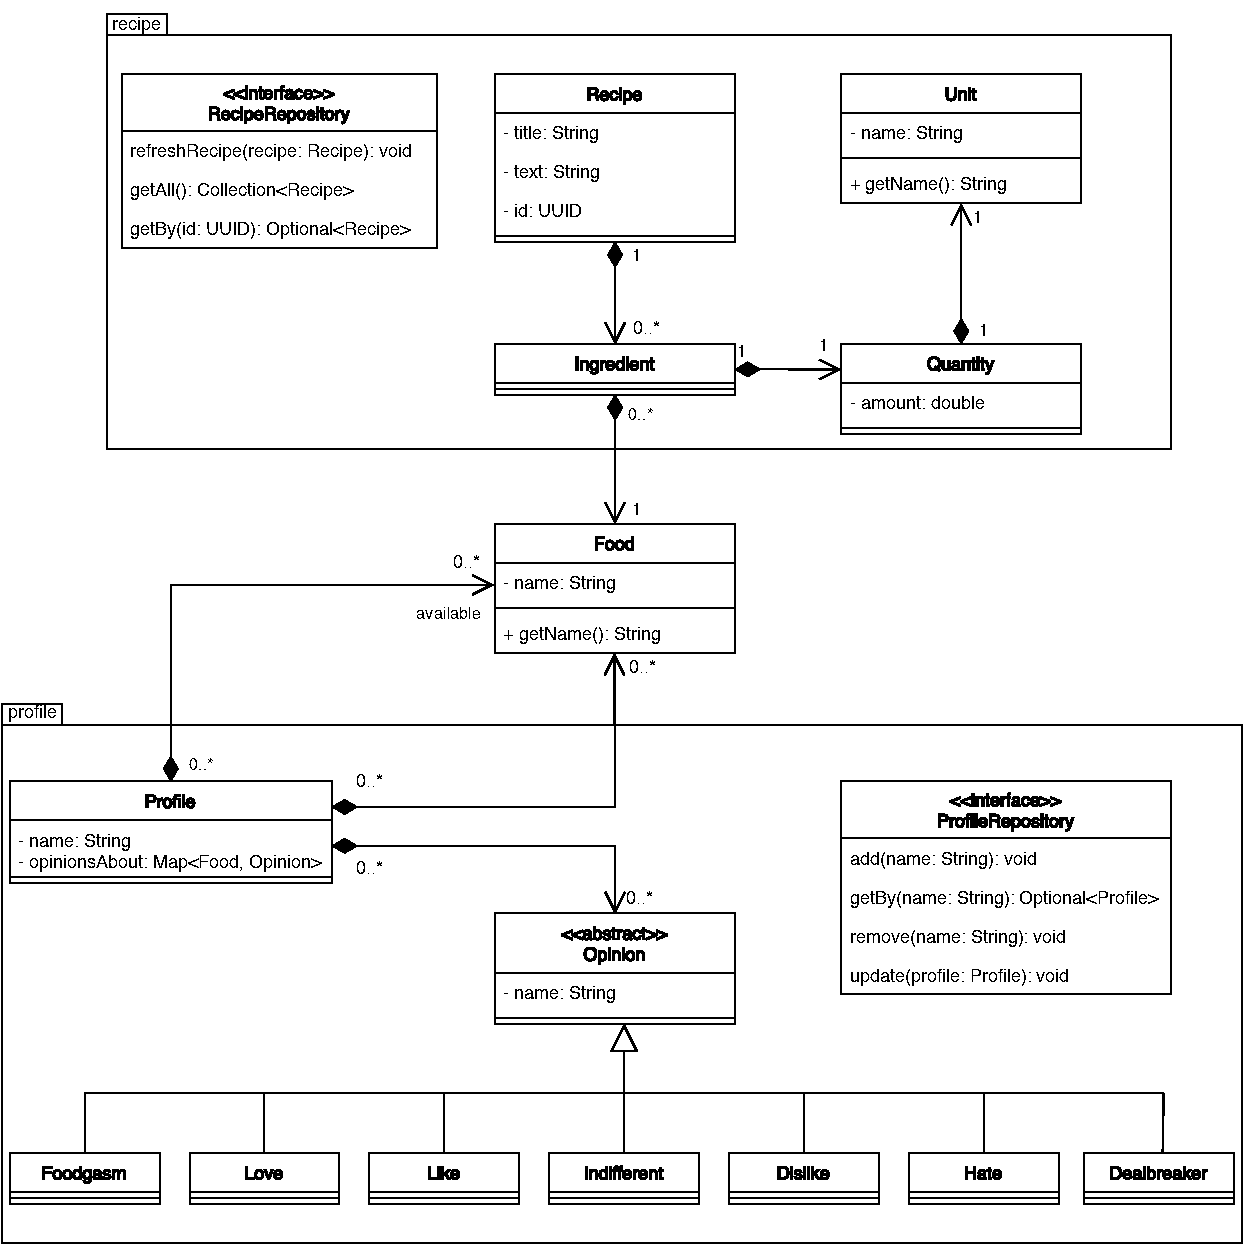
\includegraphics[width=0.98\columnwidth]{../diagrams/domain_uml.pdf}
    \caption{Klassendiagramm der Domäne}
    \label{fig:class-diag-domain}
\end{figure}

\autoref{fig:class-diag-domain} zeigt das Klassendiagramm der Domäne. Im Package \href{https://github.com/anditru/quickie/tree/bb41442c7f1ffbfcd3117cd86a40f7932e543a33/3-quickie-domain/src/main/java/org/pinkcrazyunicorn/quickie/domain/recipe}{\code{recipe}} existiert eine Entity, das Recipe. Jedes Recipe besitzt durch den Inhalt des Attributes \code{origin} eine eigene Identität. Außerdem können Rezepte in seltenen Fällen auch nachträglich abgewandelt werden und besitzen daher grundsätzlich veränderliche Werte. Bei der Ingredient hingegen handelt es sich um ein Value Object, da diese keine eigene Identität besitzt. Existieren zwei Ingredients mit dem gleichen Food und der gleichen Quantity, so sind diese gleich. Außerdem ist ihr Zustand unveränderlich, so wird etwa bei einer Änderung in einem Rezept die betreffende Ingredient gelöscht und eine neue erstellt. Ebenso verhält es sich mit der Quantity: Sind Amount und Unit einer Quantity gleich, so sind auch die Quantities gleich und auch der Zustand von Quantities ist unveränderlich. Zuletzt enthält das Package noch die Unit. Auch hier handelt es sich um ein Value Object, da auch die Gleichheit von Units lediglich von ihren Werten, also von ihren Namen abhängt. Ebenso besitzt eine Unit keinen eigenen Lebenszyklus und ihr Zustand ist unveränderlich.

Auch im Package \href{https://github.com/anditru/quickie/tree/bb41442c7f1ffbfcd3117cd86a40f7932e543a33/3-quickie-domain/src/main/java/org/pinkcrazyunicorn/quickie/domain/recipe}{\code{profile}} existiert eine Entity, das Profile. Jedes Profile besitzt durch seinen Namen eine eigene Identität, da auch zwei Profiles mit gleichem vorhandenen Food und gleichen Opinions zu verschiedenen Nutzern gehören können und daher unterscheidbar sein müssen. Auch die Unterklassen der abstrakten Klasse Opinion, welche die möglichen Opinions eines Nutzers über ein Food abbilden, sind Value Objects, da sie weder eine eigene Identität noch veränderliche Werte besitzen.

Zwischen den beiden Packages steht das Food, da es sowohl vom Profile als auch von der Ingredient verwendet wird und daher keinem der Packages eindeutig zugeordnet werden kann. Auch bei Food handelt es sich um ein Value Object, da es ebenfalls nur durch seine Werte definiert wird: Zwei Foods mit gleichem Namen sind gleich, daher besitzt es keine eigene Identität und da sich der Name auch nicht ändern wird, besitzt es auch keinen erkennbaren Lebenszyklus. 

\section{Aggregates}
Da alle Klassen im Package \href{https://github.com/anditru/quickie/tree/bb41442c7f1ffbfcd3117cd86a40f7932e543a33/3-quickie-domain/src/main/java/org/pinkcrazyunicorn/quickie/domain/recipe}{\code{recipe}} Eigenschaften eines Recipe abbilden, werden diese, also Recipe, Ingredient, Unit, Quantity und Unit, zu einem Aggregate zusammengefasst. Die Root Entity ist dabei das Recipe selbst.

Ähnlich verhält es sich im Package \href{https://github.com/anditru/quickie/tree/bb41442c7f1ffbfcd3117cd86a40f7932e543a33/3-quickie-domain/src/main/java/org/pinkcrazyunicorn/quickie/domain/profile}{\code{profile}}: Auch hier bilden alle Klassen direkt oder indirekt Eigenschaften des Profiles ab, daher werden auch diese, also Profile und Opinion bzw. deren Unterklassen zu einem Aggregate zusammengefasst. Die Root Entity ist hier das Profile.

Das Food nimmt eine Sonderstellung ein: Da sie von beiden Aggregates verwendet wird und daher zuvor auch schon keinem Package eindeutig zugeordnet werden konnte, ist sie Teil beider Aggregates.

\section{Repositories}
Für den Zugriff auf den persistenten Speicher werden zwei Repositories gemäß dem Grundsatz \enquote{Ein Repository pro Aggregate} definiert: Das ProfileRepository erlaubt den Zugriff auf das Profile, also die Root Entity des entsprechenden Aggregates. Analog hierzu ermöglicht das RecipeRepository Zugriff auf das Recipe als Root Entity des zugehörigen Aggregates. 

\chapter{Clean Architecture}
In diesem Kapitel wird die Architektur der entwickelten Software beschrieben. Diese wurde nach den in der Vorlesung besprochenen Prinzipien der Clean Architecture aufgebaut. Jeder der nachfolgenden Abschnitte behandelt dabei eine Schicht. In der Implementierung entspricht den Schichten 1, 2 und 3 jeweils ein Java-Module. Lediglich Schicht 0, welche die Plugins und das Main-Module mit der Main-Klasse der Applikation enthält, bildet eine Ausnahme: Hier entspricht jedem Plugin sowie dem Main-Module eine separates Java-Module, da diese komplett und leicht austauschbar sein sollen.

Die Clean Architecture hält neben den vier für dieses Projekt verwendeten Schichten noch eine fünfte bereit, den Abstraction Code. Auf diese Schicht, wurde für dieses Projekt jedoch verzichtet, da für die in der Domäne behandelten Themengebiete \enquote{Kochrezepte} und \enquote{Lebensmittel} kein domänenübergreifendes Wissen notwendig war, welches Teil dieser Schicht hätte sein müssen. 

\section{Schicht 3: Domain}
In dieser Schicht wurde der Domain Code der Software implementiert. Dieser befindet sich im Module \code{3-quickie-domain}, welches als solches frei von jeglichen Abhängigkeiten ist.

Sie enthält als zentrale Schicht der Clean Architecture alle Entities und Value Objects, welche die Enterprise Business Logik der Software implementieren sowie die Interfaces für die zugehörigen Repositories. Ihr genauer Inhalt ist in \autoref{fig:class-diag-domain} dargestellt.

\section{Schicht 2: Application}
Der Application Code der Software wurde in dieser Schicht implementiert und befindet sich im Module \code{2-quickie-application}, welches lediglich eine Abhängigkeit auf die zuvor beschriebene Schicht 0 besitzt.

\begin{figure}[ht!]
    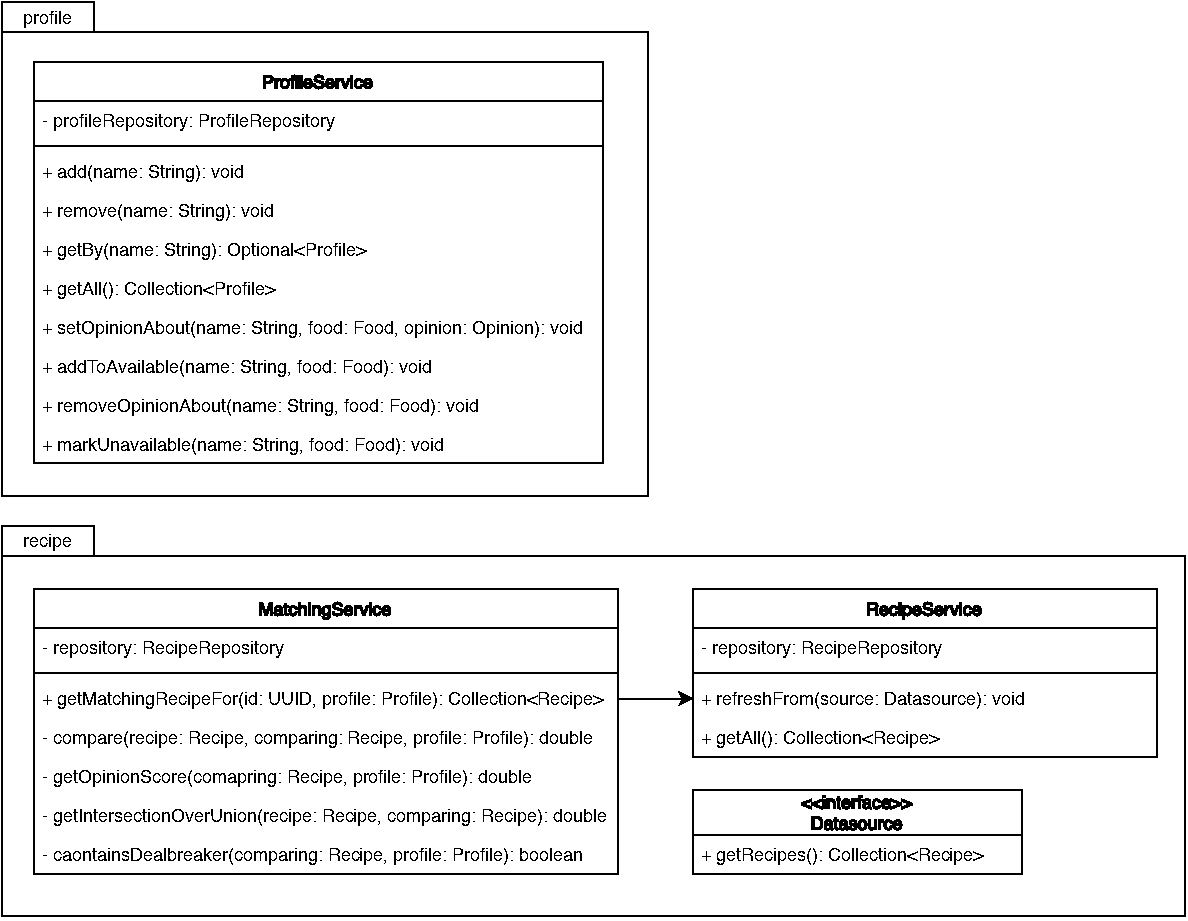
\includegraphics[width=0.98\columnwidth]{../diagrams/application_uml.pdf}
    \caption{Klassendiagramm der Applikationsschicht}
    \label{fig:class-diag-application}
\end{figure}

Sie Implementiert die eingangs beschriebenen Anwendungsfälle gruppiert in den drei Services \code{ProfileService}, \code{MatchingService} und \code{RecipeService}. Diese sind in \autoref{fig:class-diag-application} als Klassendiagramme dargestellt. Die einzige Abhängigkeit besteht dabei auf den Domaincode der Software.

\section{Schicht 1: Adapters}
Die Adapterschicht wurde im Module \code{1-quickie-adapters} implementiert und erfüllt in der zugrundeliegenden Software zwei Aufgaben: Zum einen werden die Daten durch Mapper-Klassen von dem Format, welches die Services aus der Applikationsschicht liefern, in das Format übersetzt, welches die Plugins benötigen und umgekehrt. Zum anderen regelt sie die Kommunikation zwischen den Plugins und der Applikationsschicht. Um hierbei eine möglichst große Entkopplung zwischen den Plugins und Applikationsschicht zu erreichen, geschieht diese Kommunikation eventbasiert.

\begin{figure}[ht!]
    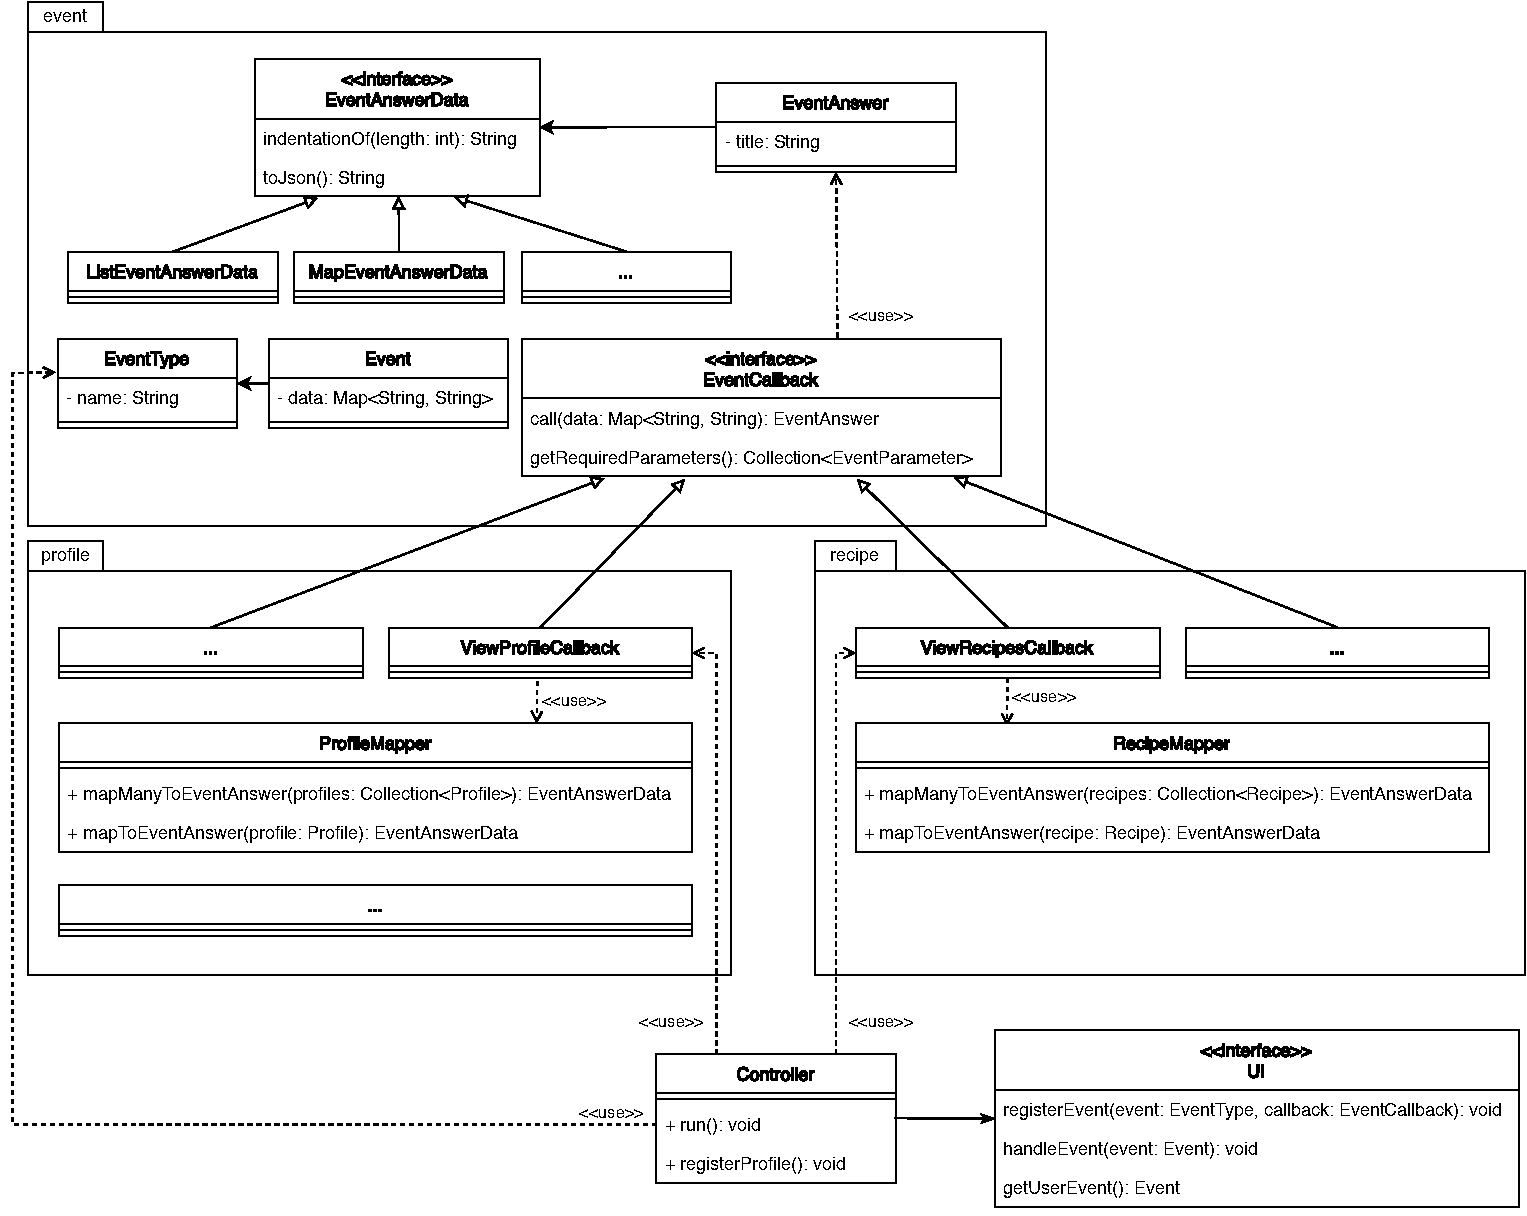
\includegraphics[width=0.98\columnwidth]{../diagrams/adapter_uml.pdf}
    \caption{Vereinfachter Ausschnitt des Klassendiagramms der Adapterschicht}
    \label{fig:class-diag-adapter}
\end{figure}

\autoref{fig:class-diag-adapter} zeigt einen Ausschnitt des Klassendiagramms der Adapterschicht in vereinfachter Form. Die Adapterschicht besitzt vier Packages: \code{event}, \code{profile}, \code{recipe} und \code{persistence}. Letzteres wurde hier im Sinne der Übersichtlichkeit zunächst nicht dargestellt. 

Das Package \code{event} enthält Pure Fabrication Code, welcher ausschließlich die eventbasierte Kommunikation betrifft. Die Klasse \code{Event} repräsentiert hierbei ein Event, welches von der Benutzeroberfläche gesendet wird und besitzt einen \code{EventType}. Die Klasse \code{EventAnswer} bildet das Resultat der Verarbeitung eines Events ab, welches an die Benutzeroberfläche zurückgeschickt wird. Die Daten, welche mittels der \code{EventAnswer} an die Benutzeroberfläche geschickt werden, werden in einem separaten Objekt gehalten. Hierbei handelt es sich je nach Form der Daten um eine Instanz einer Klasse, welche das Interface \code{EventAnswerData} implementiert. Die Logik, welche beim Auftreten eines bestimmten Events aufgerufen wird, befindet sich in Callback-Klassen. Zu jedem \code{EventType} existiert eine eine entsprechende Callback-Klasse, welche das Interface \code{EventCallback} implementiert.

In den Packages \code{profile} und \code{recipe} werden zum einen die entsprechenden Callback-Klassen implementiert und zum anderen Mapper-Klassen, welche die von der Applikationsschicht erhaltenen Daten in das von der Benutzeroberfläche benötigte Format überführen.

Das zentrale Element der Adapterschicht ist der Controller. Dieser registriert beim Start der Applikation zunächst für jeden \code{EventType} die zugehörige Callback-Klasse bei der Benutzeroberfläche, welche das Interface \code{UI} implementieren muss. Er bildet außerdem den Einstiegspunkt bei der Verarbeitung eines Events von der Benutzeroberfläche, indem er das aufgetretene Event von der Benutzeroberfläche abfragt und dessen Verarbeitung durch den Aufruf der Methode \code{handleEvent} in Gang setzt. 

\begin{figure}[ht!]
    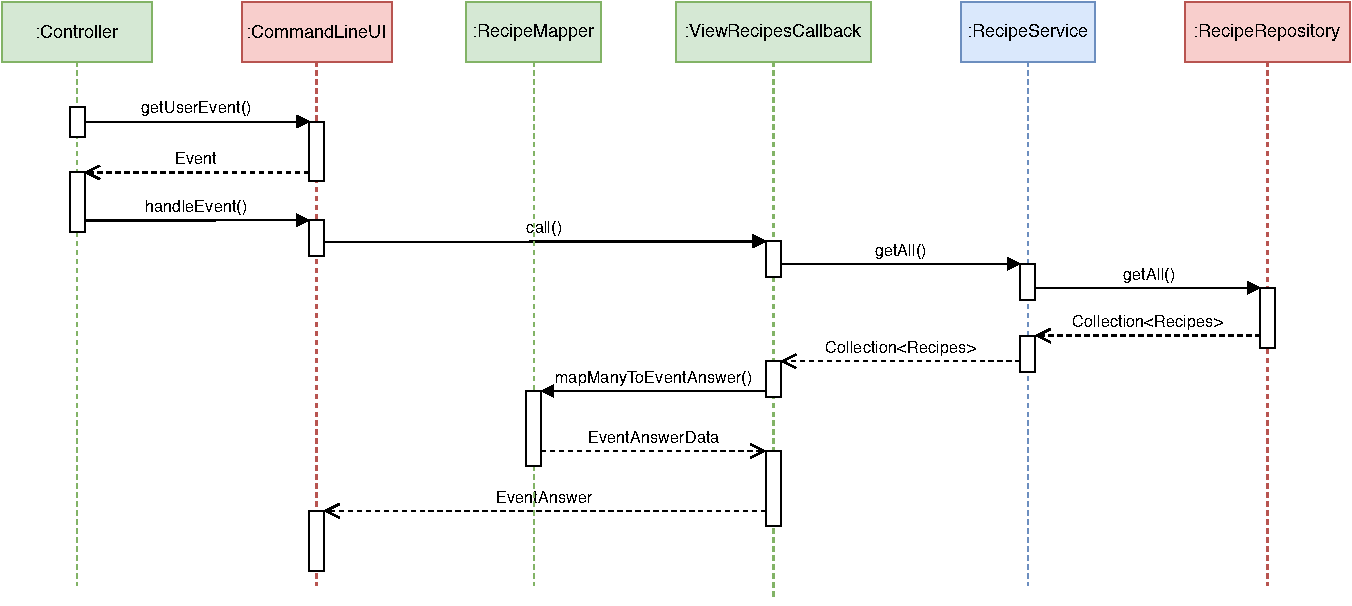
\includegraphics[width=0.98\columnwidth]{../diagrams/adapter_sequence.pdf}
    \caption{Verarbeitung eines User-Events}
    \label{fig:squence-diag-adapter}
\end{figure}

\autoref{fig:squence-diag-adapter} zeigt beispielhaft den Ablauf bei der Verarbeitung eines Events vom Typ \code{viewRecipes}. Die beteiligten Objekte sind hier farblich nach ihrer Schichtzugehörigkeit markiert: Grün steht für die Adapterschicht, Blau für die Applikationsschicht und Rot für ein Plugin.

Das Package \code{persistence} bildet die Schnittstelle zwischen der Applikationsschicht und Plugins für die Persistenz. Hier werden Interfaces definiert, welche die zu persistierenden Klassen implementieren müssen, nämlich \code{PersistentProfile}, \code{PersistentRecipe} und \code{PersistentIngredient}. Außerdem werden die Mapper-Klassen \code{PersistentProfileMapper} und \code{PersistenRecipeMapper} implementiert, welche die Domänenobjekte in ihre persistenten Gegenstücke transformieren und umgekehrt. Ferner werden in dem Package die Interfaces \code{PersistentProfileFactory} und \code{PersistentRecipeFactory} definiert, welche dann im Persistenz-Plugin implementiert werden und in den Mapper-Klassen verwendet werden, um leere \code{PersistentProfile}s und \code{PersistentRecipe}s zu erzeugen. Zuletzt werden hier auch die beiden im Domaincode definierten Interfaces \code{RecipeRepository} und \code{ProfileRepository} in den beiden abstrakten Klassen \code{PersitentRecipeRepository} und \code{PersistentProfileRepository} implementiert, von welchen dann die Repositories in einem Persistenz-Plugin erben.

\section{Schicht 0: Plugins und Main}

\subsection{Plugin \acs{CLI}}
Dieses Plugin, welches im Module \code{0-quickie-plugin-cli} implementiert wurde und die Benutzeroberfläche der Software bildet, enthält lediglich die Klasse \code{CommandLineUI}. Diese implementiert das Interface \code{UI} aus der Adapterschicht. Abgesehen von dieser besitzt dieses Plugin nur eine weitere Abhängigkeit: Die Library Apache Commons \acs{CLI}, welche zur leichteren Implementierung der \ac{CLI} verwendet wird. Das Plugin kommuniziert lediglich über die Eventfunktionalität der Adapterschicht mit dem Kern der Software, ist damit nur sehr lose an den selben gekoppelt und kann leicht ausgetauscht werden.

\subsection{Plugin Gson}

\subsection{Plugin JPA}
Dieses Plugin wurde im Module \code{0-quickie-plugin-jpa} realisiert die Persistenz der Software mit Hilfe der \ac{JPA} und deren Implementierung Hibernate. Auch dieses Plugin besitzt nur eine Abhängigkeit auf die Adapterschicht, da hier die dort im Package \code{persistence} definierten Interfaces für Factories und die zu persistierenden Objekte Recipe, Ingredient und Profile implementiert werden. Letztere enthalten außerdem die \ac{JPA}-Annotationen. Ferner enthält das Plugin die Klassen \code{JPARecipeRepository} und \code{JPAProfileRepository}, welche von den beiden abstrakten Repository-Klassen aus der Adapterschicht erben. Schließlich enthält das Plugin noch den \code{PersistenceMananger}, einen Singleton, welcher den \code{EntityManager} von \code{JPA} für die Repositories liefert.

\subsection{Plugin Scraper}
In diesem Plugin wird die Extraktion der Rezepte aus den entsprechenden Webseiten im Module \code{0-quickie-plugin-scraper} implementiert. Hierzu werden die Webseiten zunächst durch den \code{CachedDownloader} heruntergeladen. Für das Parsen der Webseiten wird der \code{HensslerScraper} verwendet, welcher die Rezeptdaten aus dem HTML-Text extrahiert. Diese werden dann durch die \code{HensslerDatasource}, welche das in der Applikationsschicht definierte Interface \code{Datasource} implementiert, für die Applikationsschicht zugänglich gemacht. Die Daten durchlaufen damit nicht die Adapterschicht, da der Scraper die Daten problemlos direkt in dem von der Applikationsschicht benötigten Format liefern kann.

\subsection{Main}
Das Module \code{0-quickie-main} enthält lediglich die Main-Klasse der Applikation, welche alle nötigen Klassen instanziiert und ggf. injected. Zuletzt wird hier auch die Methode \code{run} des Controllers aus der Adapterschicht ausgeführt und somit die Verarbeitung von Events gestartet. Dieses Modul besitzt folglich Abhängigkeiten auf alle anderen Modules der Software und befindet sich daher in der äußersten Schicht.


% ---- Anhang
\appendix
%\clearpage
%\pagenumbering{Roman}  % römische Seitenzahlen für Anhang

\newpage
\end{document}
